We used a bag-of-words approach exploiting a technique called Latent Semantic Analysis (also known as Latent Semantic Indexing), formalized by Scott Deerwester et al. in 1990\cite{LSA}. LSA is an information retrieval statistical approach, that can be used to find semantic similarities between sets of documents. It takes advantage of Singular Value Decomposition on a vector space of term frequencies in order to create, given a set of documents, an \emph{index} matrix, that can be queried with other documents to find the most similar one.
\\
As for the TF-IDF approach, each document is previously preprocessed and it is assumed to deal with news articles composed by separated paragraphs.
\\
Given a topic $T$ and the number of dimensions of the LSA space $dim$, our implementation returns the $p$ most similar paragraphs to each sentiment shift. The training of the model is performed on the whole corpus of tweets of the topic, while the similarity of a paragraph to the shift is computed as the sum of the similarities w.r.t. each tweet belonging to the latter.
\\\\
\begin{algorithmic}
\STATE \textbf{LSA Method}($T$,$dim$,$p$)
\STATE
\STATE $LSA$.train($Tweets_T$,$dim$)
\STATE
\FORALL {$S \in Shifts_T$}
	\FORALL {$Article \in News_{T,S}$}
		\FORALL {$Paragraph \in Article$}
			\STATE $simVector$ $\leftarrow$ $LSA$.index($Tweets_{T,S}$,$Paragraph$)
			\STATE $similarity$($Paragraph$) $\leftarrow$ $\sum_{x \in simVector} x $
		\ENDFOR
	\ENDFOR
	\STATE $summaries$($S$) $\leftarrow$ the $p$ paragraphs with higher $similarity$

\ENDFOR
\STATE
\RETURN $summaries$

In figure \ref{fig:LSI} is represented the work-flow of the algorithm 

\begin{figure}[htbp]
	\centering
			{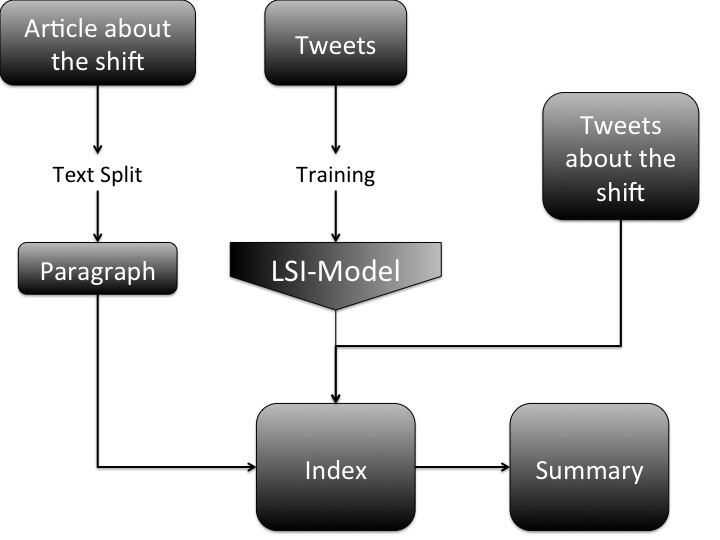
\includegraphics[width=8.5cm,height=7cm]{image/LSI.jpg}}	
		\caption[LSI]{Graphical representation of LSI algorithm}
	\label{fig:LSI}
\end{figure} 

\end{algorithmic}
